\subsubsection{Rancangan Detail Node}
\label{subsubsection:detail-node}

Seperti yang sudah dijelaskan pada bagian \ref{subsubsection:node}, \textit{Node} merupakan satuan fungsional utama yang berperan sebagai entitas dalam sistem \textit{database} terdistribusi yang dikembangkan. Selain komponen yang telah disebutkan pada bagian tersebut, \textit{Node} juga memiliki komponen internal yang berfungsi untuk menghasilkan data \textit{trace} yang dapat digunakan untuk keperluan \textit{debugging} dan analisis kinerja sistem serta konfigurasi yang mengatur perilaku \textit{Node}. Ilustrasi struktur \textit{Node} yang lebih detail dapat dilihat pada gambar \ref{fig:node-structure}.

\begin{figure}[ht]
    \centering
    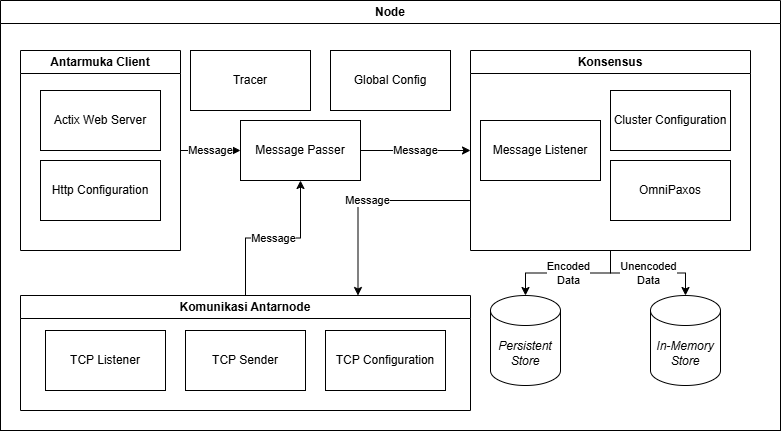
\includegraphics[width=0.95\textwidth]{resources/chapter-3/node-architecture.png}
    \caption{Struktur Node}
    \label{fig:node-structure}
\end{figure}

Komponen internal lain dalam \textit{Node} adalah jalur komunikasi \textit{message passing} antara antarmuka \textit{client}, antarmuka antar-\textit{Node}, dan komponen konsensus. Hal ini disebabkan karena modularitas implementasi OmniPaxos yang tidak mengintegrasikan komponen konsensus dengan antarmuka jaringan.

Implementasi \textit{erasure coding} bukan terdapat pada \textit{Node} melainkan pada komponen OmniPaxos. Alasan untuk hal ini adalah kompleksitas perubahan dari konsensus yang perlu dilakukan ketika operasi diubah menjadi menggunakan \textit{erasure coding}. Dengan demikian, komponen OmniPaxos akan menangani operasi \textit{erasure coding} dan replikasi data, sementara \textit{Node} akan menerima hasil dari OmniPaxos untuk melanjutkan operasi ke penyimpanan data dan komunikasi antar-\textit{Node}. Detail implementasi \textit{erasure coding} akan dibahas pada bagian \ref{subsubsection:detail-komponen-konsensus}.